\documentclass[10pt,a4paper]{article}
\usepackage[utf8]{inputenc}
\usepackage{amsmath, amsfonts, amssymb, amsthm}
\usepackage{mathtools, array, enumitem, xcolor}
\usepackage[margin=0.7in]{geometry}


\usepackage[czech]{babel}
\usepackage[utf8]{inputenc}

\theoremstyle{plain}
\newtheorem{veta}{Věta}
\theoremstyle{definition}
\newtheorem{definice}[veta]{Definice}

\setlength{\parindent}{0em}

\title{Příprava na zkoušku z DM1}
\date{}
\author{Zdeněk Tomis}

\begin{document}

\maketitle

\section{Úvod}

\section{Relace}

\begin{definice} Relace na množinách $X$ a $Y$ je podmnožina kartézského součinu $X \times Y$.
\end{definice}

\begin{definice}
Diagonální relace na $X: R = \{ (x,x):  x \in X \}$
\end{definice} 

Univerzální, prázdná

Operace s relacemi: inverze, skládání

Funkce (zobrazení) a jejich druhy: prosté (injektivní), na (surjektivní), vzájemně jednoznačné (bijektivní)

Vlastnosti relací: reflexivita, symetrie, antisymetrie, transitivita

Ekvivalence, ekvivalenční třída, rozklad množiny

\begin{definice}
Rozklad množiny X je systém disjunktních množin, jejichž sjednocení je X.
\end{definice}



Vztah mezi ekvivalencemi a rozklady (Lemma 2) 
\begin{veta}
Pro každý rozklad  $\mathcal{Q}$ množiny X je relace $\sim_\mathcal{Q}$, definovaná jako $\exists Q \in \mathcal{Q}: x,y \in Q \implies x \sim_\mathfrak{Q} y$, ekvivalencí a prvky $\mathcal{Q}$ jsou třídami ekvivalence. 
Naopak, pokud je R ekvivalence, pak $R=\sim_{\mathcal{P}(R)}$.
\begin{proof}
Reflexivita a symetrie je zřejmá. Tranzitivita jednoduše.

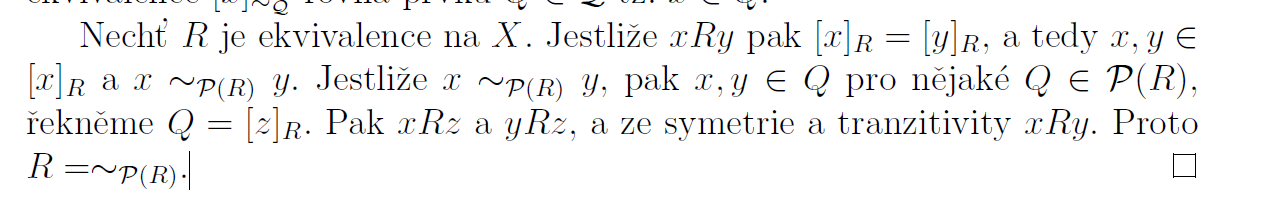
\includegraphics[scale=0.5]{ekvivalence_rozklad.png} 
\end{proof}
\end{veta}

\section{Uspořádání}

Uspořádání částečné a lineární, uspořádaná množina, ostré uspořádání

Příklady uspořádání: dělitelnost, inkluze podmnožin, lexikografické

Hasseův diagram, relace bezprostředního předchůdce

Minimální/maximální a nejmenší/největší prvek

\begin{veta}
Konečná neprázdná uspořádaná množina má minimální a maximální prvek
\begin{proof}
sporem nebo indukcí
\end{proof}
\end{veta}

Řetězec a antiřetězec

\section{Kombinatorické počítání}

\paragraph{Počet funkcí mezi množinami} $f: N \to M$ je roven $m^n$

\paragraph{Počet prostých funkcí mezi množinami} $f: N \to M$ je roven $m^{\underline{n}}$

Charakteristická funkce podmnožiny

\paragraph{Počet všech podmnožin} je rovný počtu možných charakteristických funkcí

Počet podmnožin sudé a liché velikosti
\begin{veta}
$ |\mathcal{L}| = |\mathcal{S}| $
\begin{proof}
zvolme $x$. Nechť $f(A) = A \triangle {x} =
\begin{cases} 
A \cup \{x\}  	   & \text{pokud } x \notin A \\ 
A \setminus \{x\} & \text{pokud } x \in A  \\
\end{cases}$

Toto zobrazení je bijekce: $\mathcal{L} \to \mathcal{S}$ a $\mathcal{S} \to \mathcal{L}$. Dle prinicpu bijekce $|\mathcal{L}| = |\mathcal{S}|$
\end{proof}
\end{veta}

\paragraph{Počet permutací na množině} je roven $n!$

\paragraph{Počet uspořádaných k-tic bez opakování a k-prvkových podmnožin} počet uspořádaných k-tic je roven $n^{\underline{k}}$, k-prvkových podmnožin $\binom{n}{k}$

\begin{proof}
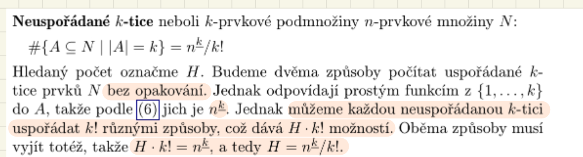
\includegraphics[scale=1]{binom.png} 
\end{proof}

Notace pro množinu všech k-prvkových podmnožin

Kombinační číslo (binomický koeficient), Pascalův trojúhelník

\paragraph{Základní vlastnosti kombinačních čísel} \begin{enumerate}
\item $\binom{n}{0} = \binom{n}{n} = 1$
\item $\binom{n}{1} = \binom{n}{n-1} = n$
\item $\binom{n}{k} = \binom{n}{n-k}$
\item $\binom{n}{k} = \binom{n-1}{k-1} + \binom{n-1}{k}$
\item $\displaystyle \sum_{i=0}^n \binom{n}{i} = 2^n$
\end{enumerate}

Binomická věta
\begin{veta}[Binomická]
$(x+y)^n = \displaystyle \sum^n_{k=0} \binom{n}{k} x^{n-k}y^k$
\begin{proof}
$(x+y)^n =\underbrace{(x+y)(x+y)...(x+y)}_{n-\text{krát}}$

Každý člen $n^{n-k}y^k$ je tam $\binom{n}{k}$-krát.
\end{proof}
\end{veta}

Princip inkluze a exkluze
\begin{veta}[PIE]
Nechť $A_1, ..., A_n$ je systém podmnožin X, t. ž. $\forall x \in X: \exists i: x \in A_i$. Potom
\[ \left|\bigcup^n_{i=1} A_i	\right| = \sum^n_{k=1} (-1)^{k-1} \sum_{I \in \binom{[n]}{k}} \left| \bigcap_{i \in I} A_i \right| = \sum_{\emptyset \neq I \subseteq [n]} (-1)^{|I|-1} \left| \bigcap_{i \in I} A_i \right| \] 
\begin{proof}
Pro libovolné $x \in X$.
Nechť $j$... počet množin obsahujících x.

přečísluju $A_1, ..., A_j$

Na levé straně věty se $x$ objeví právě jednou.

Na pravé straně se objeví:
$\# = j - \binom{j}{2} + \binom{j}{3} - ... \pm \binom{j}{j} = 1 -(1-1)^j  = 	 1$
\end{proof}
\end{veta}

Problém šatnářky: počet permutací bez pevného bodu
\begin{veta}[Problém šatnářky]
Šatnářka rozdá každému špatný kloubouk s pravděpodobností ... .
\begin{proof}
Rozdělme si všechny permutace do podmnožin s alespoň jedním pevným bodem j: $A_j = \{ \pi \in S_n | \pi(j) = j \}$.

Jejich sjednocením získáme permutace s alespoň jedním pevným bodem.

$|A_j| = (n-1)!$  

$|A_j \cap A_i| = (n-2)!$

$\vdots$

$\#$ permutací s alespoň jedním pevným bodem $= \displaystyle \sum^n_{k=1} (-1)^{k-1} \binom{n}k (n-k)! = n! \sum^n_{k=1} (-1)^{k-1} \frac{1}{k!}$

$\#$ permutací s bez pevného bodu $= n!(\frac{1}{2!}-\frac{1}{3!}+\frac{1}{4!} +  ... + (-1)^n \frac{1}{n!})$

Toto konverguje k $e^{-1}$

\end{proof}
\end{veta}

\section{Grafy}

Graf, vrchol, hrana, V(G), E(G)

Standardní grafy: úplný, prázdný, cesta, kružnice

Bipartitní graf, úplný bipartitní graf

Isomorfismus grafů

Stupeň vrcholu, k-regulární graf, skóre grafu

\begin{definice}
$k$-regulární graf je takový graf, jehož libovolný podgraf obsahuje vrchol stupně $k$ nebo nižší.
\end{definice}

\begin{definice}
Skoré grafu je neklesající posloupnost stupňů jeho vrcholů.
\end{definice}

Vztah mezi součtem stupňů a počtem hran, princip sudosti

Podgraf, indukovaný podgraf

Cesta, kružnice, sled a tah v grafu

Souvislý graf, relace dosažitelnosti (ekvivalence), komponenty souvislosti

\begin{veta}
Relace dosažitelnosti je ekvivalence.
\begin{proof}
Symetrie a reflexivita je zřejmá. Tranzitivita: Spojíme cesty, najdeme první vrchol zkraje, který se vyskytuje dvakrát, a odstraníme jej spolu se všemi vrcholy sledu až do opakování vrcholu. Získáme tak cestu.
\end{proof}
\end{veta}

Dosažitelnost sledem je totéž jako dosažitelnost cestou

Matice sousednosti

*Počet sledů délky k lze získat z k-té mocniny matice sousednosti

\begin{veta}
Počet sledů délky k lze získat z k-té mocniny matice sousednosti
\end{veta}

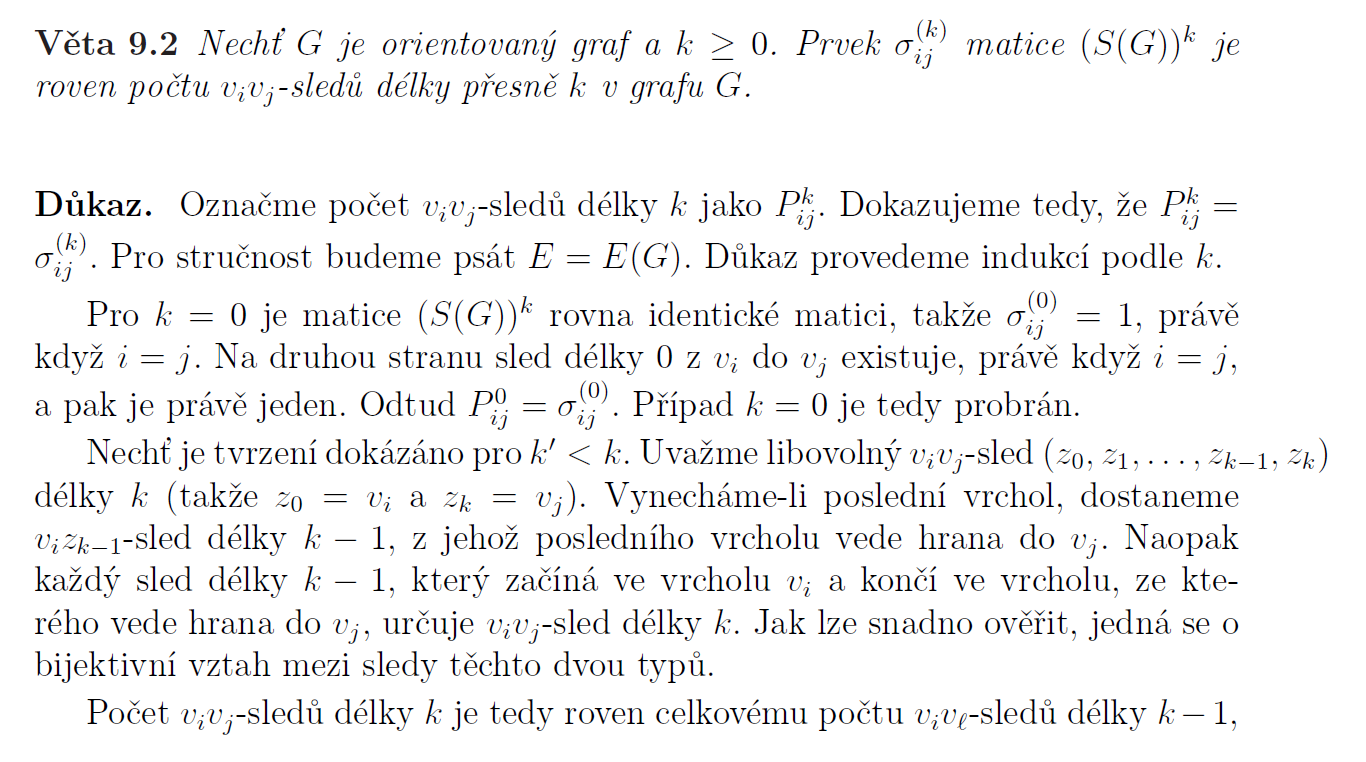
\includegraphics[scale=0.5]{sousednosti.png} 

*Vzdálenost v grafu (grafová metrika)

\begin{definice}
Grafové metriky splňují následující podmínky:\begin{itemize}
\item $v(x, y) \geq 0$
\item $v(x, y) = 0 \implies x = y$
\item Trojúhelníkové nerovnosti: $v(x, y) \leq v(x, z) + v(z, y)$
\end{itemize}
\end{definice}

*Trojúhelníková nerovnost pro vzdálenost

Grafové operace: přidání/odebrání vrcholu/hrany, dělení hrany, kontrakce hrany

Dělení hrany

Kontrakce hrany

Otevřený a uzavřený eulerovský tah

Věta o existenci uzavřeného eulerovského tahu

\begin{veta}
Graf má uzavřený eulerovský tah právě tehdy, když je  eulerovský (souvislý a všechny jeho vrcholy mají sudý stupeň).
\begin{proof}
$\implies$ 

Tah každý vrchol navštíví alespoň jednou. Každé dva vrcholy jsou spojeny podtahem, tudíž graf je souvislý. Navštívi-li tah vrchol $v-$krát, pak jeho stupeň je $2v$, tedy sudý. Graf je eulerovský.

$\impliedby$

Indukcí.

Nalezneme libovolnou hranu ${u,v}$. Po odebrání je graf stále souvislý, kdyby nebyl souvislý, neplatil by v komponentách princip sudosti, což nelze (z každé bychom odebrali jeden stupeň). Tedy nalezneme druhou cestu mezi u, v. Odebereme celou tuto kružnici. Graf se rozpadne na komponenty souvislosti. Každý vrchol v každé bude mít stupeň sudý, protože jsem od každého vrcholu odebrali sudý počet hran. Tyto komponenty tedy mají eulerovský tah a eulorevský tah původního grafu získáme napojením tahů na tah odebrané kružnice.
\end{proof}
\end{veta}

*Orientovaný graf, podkladový graf, vstupní a výstupní stupeň, vyváženost vrcholu

\begin{definice}
Vrchol orientovaného grafu je vyvážený, pokud je jeho vstupní a výstupní stupeň stejný.
\end{definice}

*Silná a slabá souvislost orientovaných grafů

*Uzavřené eulerovské tahy v orientovaných grafech

Skóre grafu (znovu výše)

Věta o skóre
\begin{veta}
$D = v_1, ..., v_n$ je skóre grafu právě tehdy, když je $D^\prime = v_1, ...,v_{n - v_n - 1}, v_{n - v_n} -1 ,..., v_{n-2} - 1, v_{n-1} - 1$ skóre grafu.
\begin{proof}
\begin{enumerate}
\item $\impliedby$

Jednoduše připojíme nový vrchol stupně $v_n$ a $v_n$ hran do předcházejících vrcholů
\item $\implies$

Složitě:

Definujme třídu grafů $\mathcal{G}$ jako všechny grafy se skóre D.

Definujme $j(G) =$ nejvyšší i, t. ž. $v_nv_i \notin E(G)$. (První vrchol zprava, se kterým nesousedí poslední.) 

Nechť $G_0$ v $\mathcal{G}$ je graf s minimálním j.

Tvrdíme, že $j(G_0) = n - v_n -1$.

Pro spor:  $j(G_0) > n - v_n -1$.

Potom $v_n$ sousedí s nějakým $v_i, i < j(G_0)$

Navíc musí existovat $v_k$, kterého $v_j$ vidí, ale $v_i$ nevidí, protože i má méně, nebo stejně sousedů, ale jeden už je $v_n$.

Můžeme prohodit $v_k v_j$ a  $v_n v_i$ za $v_n v_j$ a  $v_k v_i$ a snížíme j. To je spor s minimálním j.

\end{enumerate}
\end{proof}
\end{veta}

\section{Stromy}

Strom, les, list

\begin{veta}[Lemma o koncovém vrcholu]
Má-li strom alespoň dva vrcholy, pak má alespoň dva listy.
\begin{proof}
Nechť P je nejdelší cesta ve stromu. Potom jsou její konce listy, jinak není nejdelší.
\end{proof}
\end{veta}

\begin{veta}Je-li l list grafu G, pak G je strom, právě když G-l je strom.
\begin{proof}
Využijeme charakterizace stromu jako souvislého grafu bez kružnice. Přidání listu nevytvoří kružnici, stejně jako její odebrání. Souvislost není narušena, protože všechny cesty nekončící v odebraném vrcholu zůstanou zachovány.
\end{proof}
\end{veta}

\begin{veta}[Pět ekvivalentních charakteristik stromu]
\begin{enumerate}
\item T je minimálně souvislý.
\item Mezi každými dvěma vrcholy vede právě jedna cesta.
\item T je maximální graf bez kružnic.
\item T neobsahuje kružnici a má $|V(T)| - 1$ hran.
\item T je souvislý a má $|V(T)| - 1$ hran.
\end{enumerate}
\begin{proof}
\begin{itemize}
\item $(1) \implies (2)$
Sporem: Existují dvě různé cesty, liší se alespoň v jedné hraně, tuto hranu můžu odebrat a zachovám souvislost: Cesty bez této hrany zůstanou, cesty s touto hranou přesměruji přes druhou z původních cest.
\item $(2) \implies (3)$
Pridáním hrany xy vzniknou dvě cesty mezi x a y.
\item $(3) \implies (4)$
Graf je souvislý.
Souvislý acyklický graf obsahuje $|V(T)| - 1$ hran. (Důkaz - začnu s prázným grafem a propojuji komponenty. Vždy snížím počet komponent, pokračuji dokud není jedniná.)
\item $(4) \implies (5)$
Sporem: není souvislý: \[|E(T_1)| \leq |V(T_1)| -1\]
\[|E(T_2)| \leq |V(T_2)| -1\]
\[|E(T_1)| + |E(T_2)| \leq |V(T_1)| - 1 +  |V(T_2)| -1 \]
\[|E(T)| \leq |V(T)| - 2\]

Spor
\item $(5) \implies (1)$
Kdyby měl více hran, nebyl by acyklický, tudíž ani minimálně souvislý.
\end{itemize}
\end{proof}

\end{veta}

\begin{definice}
Kostra grafu je 	podgraf na všech vrcholech, který je strom.
\end{definice}

\begin{veta}
*Graf má kostru, právě když je souvislý.
\begin{proof}\begin{itemize}
$\implies$ strom je souvislý.

$\impliedby$ Lze dokázat asi třeba indukcí podle počtu hran. 
\end{itemize}
\end{proof}
\end{veta}


\section{Rovinné kreslení grafů}

\begin{definice}
Oblouk (prostá křivka) je prostá spojitá funkce $f: [0,1] \to \mathbb{R}^2$
\end{definice}

\begin{definice}
topologická kružnice (prostá uzavřená křivka) je spojitá funkce $f: [0,1] \to \mathbb{R}^2$, pro kterou platí $f(0) = f(1)$ a která je jinak prostá.
\end{definice}

\begin{definice}
rovinné nakreslení multigrafu G je:
\begin{itemize}
\item prosté zobrazení $\nu: V \to \mathbb{R}^2$
\item system křivek $\{c_e| e \in E\}$ takové, že: \begin{enumerate}
\item pro $e \in E: k(e) = {u,v} $ je $c_e$ jednoduchá křivka s konci $\nu(u)$ a $\nu(v)$
\item pro $e \in E: k(e) = {u} $ je $c_e$ jednoduchá uzavřená křivka  s koncem v $\nu(u)$
\item $\forall e\in E(G): \nu(V(G)) \cap c_e = \nu(k(e))$ (vrcholy neleží na křivkách)
\item pro různé hrany $c_e \neq c_{e^\prime}$ platí $c_e \cap c_{e^\prime} = \nu(k(e) \cap k(e^\prime))$ (křivky se kříží jen ve vrcholech, a to v těch správných)
\end{enumerate}
\end{itemize}
\end{definice}


Oblouková souvislost a její komponenty, stěna nakreslení

\begin{definice}
Oblouková souvislost je ekvivalence na $M \subseteq \mathbb{R}^2$, $x,y \in M, x \sim y \implies$ existuje jednoduchá křivka v M s krajními body x a y.
\end{definice}

\begin{definice}
Nechť $\nu, \{c_e | e \in E\}$ je rovinné nakresléní. Pak komponenty obloukové souvislosti $\mathbb{R} \setminus \bigcup_{e \in E} c_e$ se nazývají stěny nakreslení.
\end{definice}

Rovinný graf, topologický graf.

Rovinný graf je graf, který má rovinné nakreslení.
Topologický graf je graf a jeho jedno rovinné nakreslení.

Jordanova věta o kružnici (bez důkazu)

\begin{veta}[Jordanova o kružnici]
Je-li c jednoduchá uzavřená křivka, pak $\mathbb{R}^2 -c$ má právě dvě komponenty obloukové souvislosti, omezenou a neomezenou, a c tvoří jejich společnou hranici.
\end{veta}

\textbf{K5 a K3,3 nejsou rovinné.}




\begin{veta}
Hranice stěny je nakreslením uzavřeného sledu.

G je multigraf nakreslený v rovinně. c je jednoduchá křivka reprezentující $e \in E(G)$.

Pokud je $G \setminus e$ souvislý, pak c leží na hranici stěn.

Odpovídající nakreslení $G \setminus e$ má o stěnu méně.


Lemma.  $z$ je konečné sjednocení jednoduchých křivek protínajících se pouze v koncových bodech. $k$ je komponenta obloukové souvislosti. Pak: Je-li k omezená, pak z obsahuje jednoduchou uzavřenou křivku $c$, t. ž. k je podmnožinou komponenty obloukové souvislosti $\mathbb{R}^2 \setminus c$

\begin{proof}\begin{enumerate}
\item $G \setminus e$ je souvislý $\implies e$ leží na kružnici $k$.
\item V nakreslení G odpovídá k jednoduché uzavřené křivce $c_K$.
\item Jordan: $\mathbb{R}^2 - c_k$ má dvě komponenty obloukové souvislosti.
\item $c_k$ je obsažena v hranici obou komponent stěny nakreslení jsou podmnožinami těchto komponent.
\item $c$ je obsažena v hranicích dvou stěn
\item odebráním c tyto dvě stěny splynou.
\end{enumerate}

\end{proof}
\end{veta}

\paragraph{Stereografická projekce} je

zobrazení ze sféry bez severního pólu na rovinu

\begin{veta}
Graf jde nakreslit do roviny, právě když jde nakreslit na sféru.
\begin{proof}
Použijeme stereografickou projekci. Pokud je část nakreslení na severním pólu, nejdříve kouli pootočíme.
\end{proof}
\end{veta}

Vnější stěnu lze zvolit. (Každé nakreslení jde překreslit s libovolnou stěnou jako vnější)

Kreslení na další plochy: válcová plocha, torus

\begin{veta}[Kuratowski]
Graf je rovinný právě tehdy, když neobsahuje podrozdělení $K_{3,3}$ ani $K_5$
\end{veta}

\begin{veta}[Eulerova formule pro souvislé rovinné grafy]
$f + v= e + 2$
\begin{proof}
Indukcí podle počtu hran.

Základní případ: $e = v - 1$. Jedná se o strom, má jednu stěnu.

Indukční krok: TODO
\end{proof}
\end{veta}
 

Maximální rovinný graf je triangulace.


Maximální počet hran rovinného grafu

\begin{definice}
Délka stěny je počet hran sledu který odpovídá hranici nakreslení. 
\end{definice}

\begin{veta}[O maximimálním počtu hran]
\begin{proof}
Nechť $l$ je délka nejkratší stěny a $s$ je počet stěn.

\[ s \cdot l \leq 2|E(G)|  \implies s \leq \frac{2|E(G)| }l\]

Dle eulerovy formule:

\[ E(G) - V(G) + 2 \leq \frac{2|E(G)| }l\]

\[ E(G)\left(1-\frac{2}l \right) \leq  V(G) - 2 \]

\[ E(G) \leq  \frac{l}{l-2}  (V(G) - 2) \]

\end{proof}

\end{veta}

V rovinném grafu existuje vrchol stupně nejvýše 5.


\begin{veta}
Rovinný graf je 5-degenerovaný. Bez trojúhelníku 3-degenerovaný.
\begin{proof}
Plyne z $|E(G)| \leq 3|V(G)| - 6$.

$\sum deg(v) \leq 6|V(G)| - 12$

$avg deg(v) < 6 $

$\exists v: deg(v) \leq 5$

Libovolný podgraf rovinného grafu je rovinný, tudíž je 5-degenerovaný.
\end{proof}
\end{veta}


Počet hran a vrcholů nízkého stupně v rovinných grafech bez trojúhelníků

Duální multigraf
\section{Barvení grafů}

\begin{definice}
k-obarvení grafu je zobrazení $\phi: V(G) \to [k]$, t.ž. $\forall uv \in E(G): \phi(u) \neq \phi(v)$
\end{definice}

\begin{definice}
Barevnost grafu $\chi(G)$ je rovna minimálnímu $k$, t.ž. $G$ má $k-$obarvení
\end{definice}

Barevnost úplných grafů, cest a kružnic

*Ekvivalentní tvrzení: graf má barevnost nejvýše 2, graf je bipartitní, graf neobsahuje lichou kružnici. Věta 5

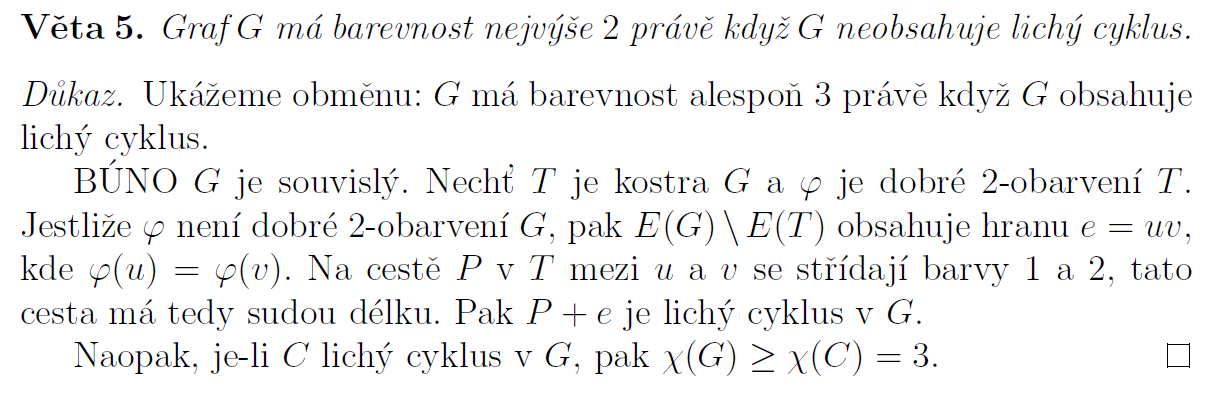
\includegraphics[scale=0.5]{bipart.png} 

*Barevnost $\geq$ klikovost Pozorování 2

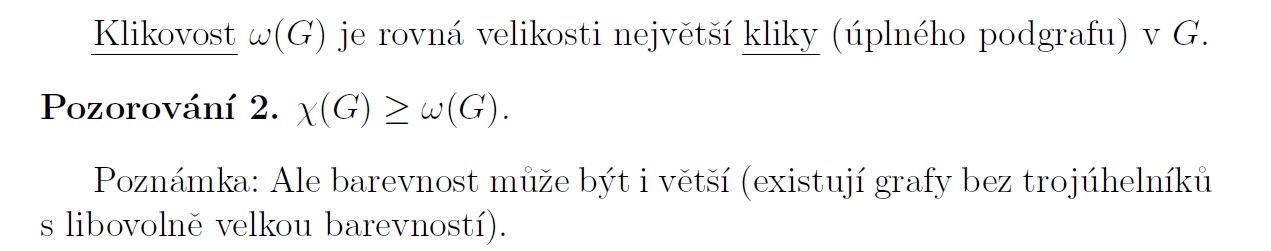
\includegraphics[scale=0.5]{klika.png} 

Princip barvení indukcí: stromy jsou 2-obarvitelné, rovinné grafy 6-obarvitelné

Barevnost $\leq$ maximální stupeň + 1 (Protože pokud $max deg = k$, pak je graf určitě k-degenerovaný)


\begin{veta}[ Věta o 5 barvách]
Každý rovinný graf má 5-obarvení.
\begin{proof}
Indukcí. Základní případ triv.

Indukční krok: Nalezneme vrchol stupně 5 nebo menší. \begin{enumerate}
\item Pokud má vrchol stupeň čtyři nebo menší, triv.
\item Najdeme dva sousedy, kteří nesousedí spolu, takoví existují, jinak je to $K_5$, což není rovinné (kuratowski). Kontrahujeme obě hrany a zahodíme násobné. Obarvíme 5 barvami, dva sousedí sdílí stejné, vybereme zbylou.
\end{enumerate}
\end{proof}
\end{veta}

*Věta o 4 barvách (bez důkazu)

\section{Pravděpodobnost}

Pravděpodobnostní prostor diskrétní, konečný, klasický

\begin{definice}
Pravděpodobnostní prostor je trojice $(\sigma, \omega = 2^\omega, P)$, kde $\sigma$ je množina elementárních jevů, $\omega$ je množina jevů a P je zobrazení $P: \omega \to [0,1]$, takové že
\end{definice}

Jev elementární, jev složený, pravděpodobnost jevu

Jev se také dá popsat logickou formulí.

*Bertrandův paradox s kartičkami

Podmíněná pravděpodobnost

\begin{veta} [Věta o úplné pravděpodobnosti]
Nechť $\Omega = \bigcup^n_{i=i} B_i$ disjunktních množin.
Poté 
\[ P[A] = P[A|B_1]\cdot P[B_1] + ... + P[A|B_n]\cdot P[B_n]\]
\begin{proof}
Úpravami
\end{proof}
\end{veta} 

\begin{veta}[Bayesova věta]
\[P[B|A] = \frac{P[A|B] \cdot P[A]}{P[B]}\]
\end{veta}



Jevy nezávislé a po dvou nezávislé

Součin pravděpodobnostních prostorů, projekce

Náhodná veličina

Logické formule s náhodnými veličinami dávají jevy.

Střední hodnota

Věta o linearitě střední hodnoty

Indikátor náhodného jevu

Použití indikátorů k výpočtu střední hodnoty

Markovova nerovnost

Velikost řezu v grafu: střední hodnota, existuje velký řez, pravděpodobnostní algoritmus 

\end{document}